\chapter{Interaction between Languages}

After providing scheme, lua support into the browser, we needed a way for this language to interact with each other. 

Every language is different, and achieving even slight levels of language interoperability is pretty difficult because the wide variation in programming language features, and implementations. after going through all the challenges and possible solution, For this project, we decided to take approach which will be similar to Nashorn \cite{Juneau2017}, code from other languages can be called by using the helper evaluate function provided by that language.

All languages will provide evaluate function, which will evaluate code native to that language and will return the results.

We will see the interaction between different languages with examples, in following sections.

\subsection{Scheme to JS Interaction}

Our implementation of scheme provides, evaluate function called "js-eval", which takes argument of java script code in string, and it executes that java script code from scheme environment, as shown in example below,

\begin{lstlisting}[frame=single]
<!DOCTYPE html>
<html>
<head>
<title>Calling Java Script from Scheme example</title>
</head>

<body>
<input type="button" id="call" 
value="Click to call Java Script from Scheme" />

</body>
<script type="text/scheme">
(
  (add-handler! "#call" "click" (lambda(ev)
    (js-eval "var sayHello = function (tmp) {
                                   return 'Hello ' + tmp
                                 };"
    )
    (js-eval "alert('Java Script Alert from Scheme - ' 
     + sayHello('Swapnil'))")))
  )
 )
</script>
\end{lstlisting}

The above code, adds a click handler to input button with id "call", after clicking a button it executes a js-eval function of scheme, which creates javascript function called sayHello, and then next line executes that Java Script function by passing arguments to it.  Output generated by above code is shown in the figure \ref{fig:scheme-js-interaction}.

\begin{figure}[H]
	\begin{center}
		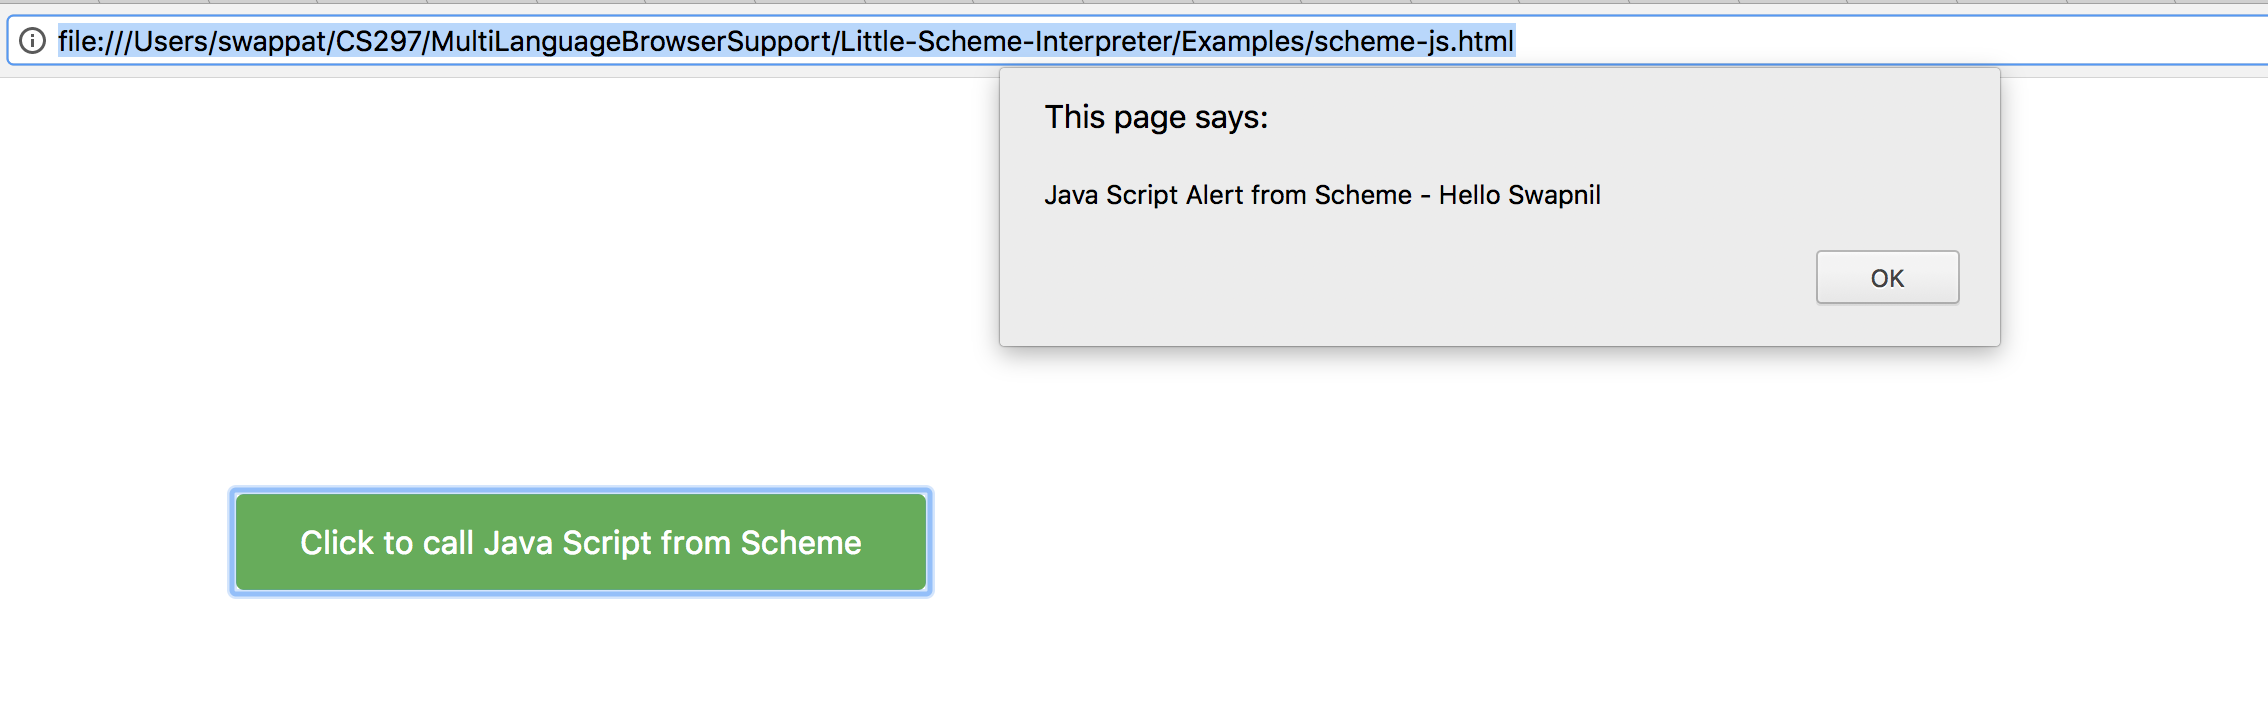
\includegraphics[width=\linewidth]{./images/scheme-js-interaction.png}
	\end{center}
	\caption{Executing Java Script from Scheme: Output}
	\label{fig:scheme-js-interaction}
\end{figure}


\subsection{JS to Scheme Interaction}

Similar, to calling Java Script code from scheme, we can also execute scheme code from java script. Web page, gets the instance of our scheme interpreter, by calling evaluate method on that instance, java script can execute scheme code, as shown in code below, 

\begin{lstlisting}[frame=single]
<!DOCTYPE html>
<html>
<head>
<meta charset="utf-8" />
<title>Calling Schemet from Java Scriptexample</title>
</head>
<body>
<input type="button" onclick="callScheme()" 
id="call" value="Execute Scheme Code from Java Script">
</body>
<script>
function callScheme()
{
 var sayHello = scheme.evaluate("(lambda (msg)  (alert msg) )");
 sayHello("Calling scheme method from Java Script!!!!!");
}
</script>
</html>
\end{lstlisting}

In the above code, we are evaluating function written in scheme, and calling it from Java Script. "scheme.evaluate" functions executes the scheme code, In this case, we are storing scheme lambda function in variable called sayHello, and calling it with parameters from Java Script, as shown in figure \ref{fig:js-scheme-interaction}

\begin{figure}[H]
	\begin{center}
		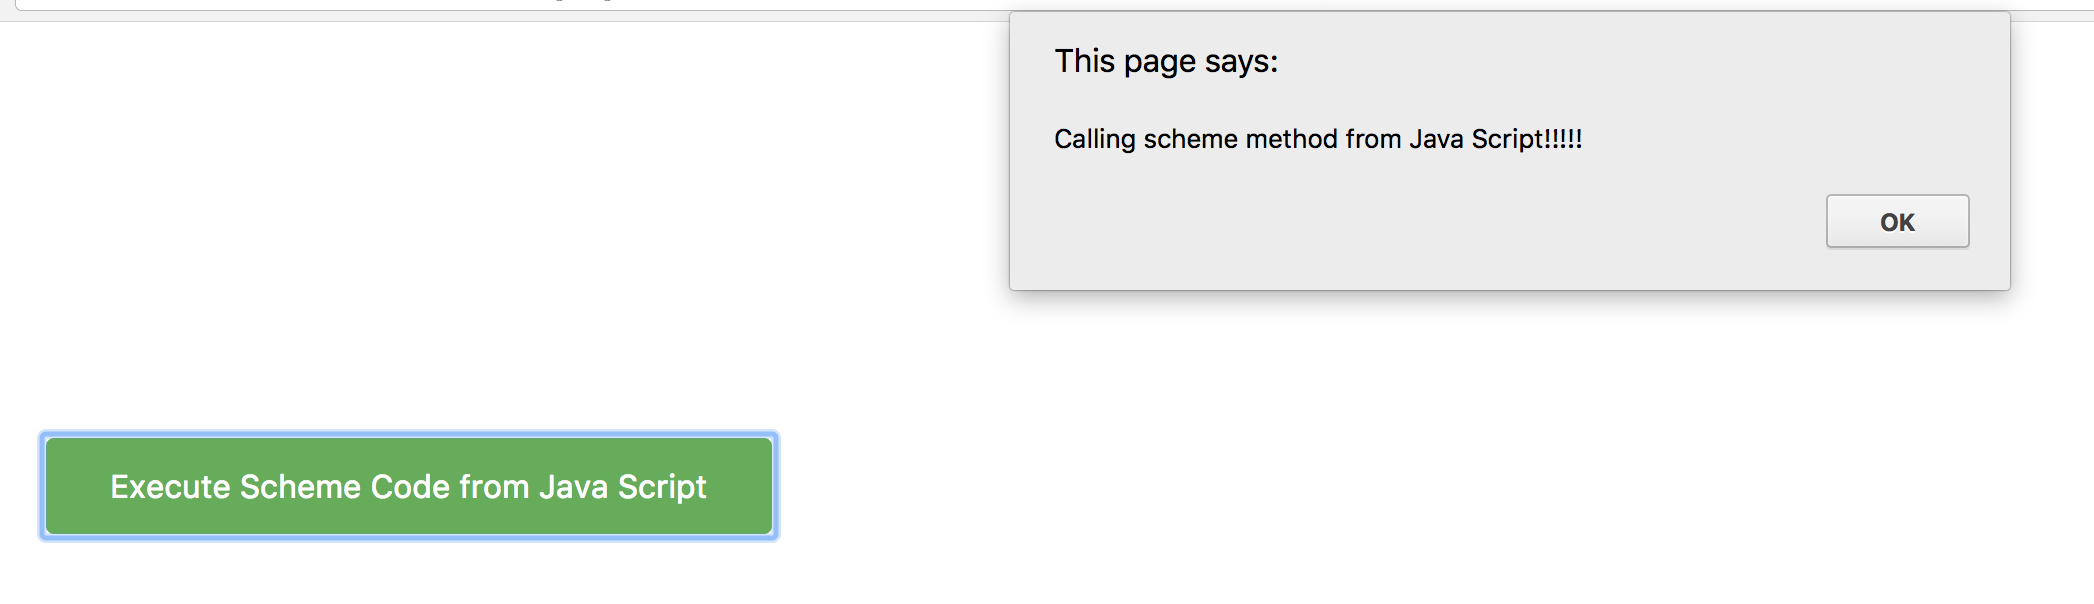
\includegraphics[width=\linewidth]{./images/js-scheme-interaction.png}
	\end{center}
	\caption{Executing Scheme from Java Script: Output}
	\label{fig:js-scheme-interaction}
\end{figure}


\subsection{Lua to JS Interaction}




\subsection{JS to Lua Interaction}
